%!TEX root = ../../thesis.tex

\section{Orbital Solutions}
\label{sec:orbtial_diagrams}
The insufficient observational spacing becomes clear when the orbits are visualized by plotting the {RV} variation.
\Crefrange{fig:hd4747p89}{fig:hd30501p89} show the {RV} curves for each target observed for this project.
The target stars that have two companions are shown twice, with each companion treated as a single Keplerian (ignoring the presence of the other companion).
For each figure the left hand plot shows the {RV} variation across a full orbit of the companion, while the plot on the right shows the {RV} variation for the 6 month observation window of {Period 89} only.
The solid black line indicates the {RV} of the host star (with scale on the left hand axis), while the blue dashed line shows the {RV} of the companion (with the scale on the right hand axis).
The orange crosses and red stars indicate on the {RV} curves the times at which observations were obtained for each target, for the host and companion respectively.

The first thing that is apparent is the variation of shape of the {RV} curves.
This is normal with the variations in shape arise from the different orbital parameters of each target (provided in \cref{tab:orbitparams}).
In the left hand plots, in which a full orbit is shown, the different shapes are created from the eccentricity, \(e\), and argument of periapsis, \(\omega\).
In the right hand panels, for which a fixed time period is shown, the orbital period of the companion also plays a role.
Specifically the ratio of orbital period to the 6 month observing period determines what fraction (or multiples) of the orbit is displayed.

The {RV} curves of the star and the planet mirror each other about the systems mean velocity, \(\gamma\), with the amplitude scaled by their mass ratio, \(q\) (see \cref{eqn:q_ratio_K2}), and \(\omega\) offset by \(180^\circ\).

All the plots, apart from {HD\,4747}, have more than one observations shown, although it can be difficult to see as there observational spacing is small.

For the companions {HD\,162020}b (\cref{fig:hd162020p89}) and {HD\,168443}b (\cref{fig:hd168443bp89}) their orbital periods are shorter than 6 months, allowing for multiple orbits to occur during {Period 89}.
As such the full amplitude range was available to measure in the observing Period if observations were taken at correct times, at the locations of the extrema.
It should have been possible to obtain observations in which the companion spectra were sufficiently separated for the differential separation technique.
However in reality, the two observations for these two targets were taken immediately after each other, making any differential extremely small.
This is ignoring the fact that the flux ratios (from \cref{tab:estimated_flux_ratios}) for these short period companions are estimated to be very low, meaning they would have been very difficult to detect even if observed at the extrema.

The larger companion {HD\,168443}c in \cref{fig:hd168443cp89} has a longer orbital period, so it appear as straight line in the right hand panel, although the amplitude variation of the companion during {Period 89} is about 8--9\kmps.
Therefore observations taken at the extreme ends of {Period 89} may have provided just enough separation to be suitable for the differential.

For HD\,202206 about 3/4 of the orbit is covered in {Period 89} with a {RV} amplitude of the companion possible of over 40\kmps{}.
Therefore, in this case well separated {RV}s could have been obtained.

For the remaining targets with long periods, it is clear that sufficiently separated {RV}s were not obtained, but also that they were not possible within a single observing period with a {RV} variation less than 6\kmps{} during {Period 89}.
For HD\,30501 the largest time separation between observations obtained is clearly visible in \cref{fig:hd30501p89}.
Unfortunately, this did not result in a large enough companion separation.
Looking at the full period, if the observations had been obtained in the previous period then sufficient separation could have possibly been obtained.

The code used to create orbital plots similar to those shown here is available under the \href{https://github.com/iastro-pt/ObservationTools}{iastro-pt/Observationtools} \emph{Github} repository with documentation available on \href{https://ia-observationtools.readthedocs.io/en/latest/rv.html}{Read the Docs}.

The sampling of points in the orbit reveal that the choice of points was not favourable for the application of the direct subtraction technique.
This was unfortunately discovered after attempting to apply the technique.

%!TEX root = ../thesis.tex
% Plotting the orbital plots for each target

\begin{figure}
    \centering
    \begin{tabular}{cc}
        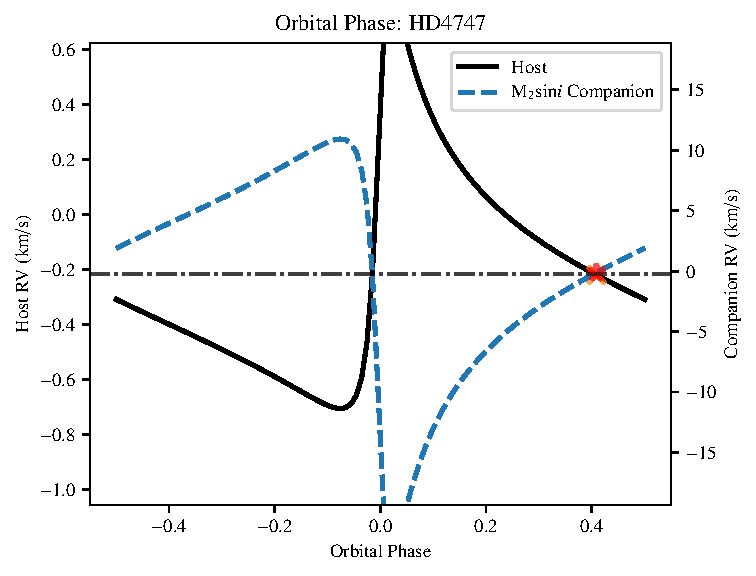
\includegraphics[width=0.45\linewidth]{figures/direct-recovery/orbital-plots/HD4747_orbital_phase.pdf} & 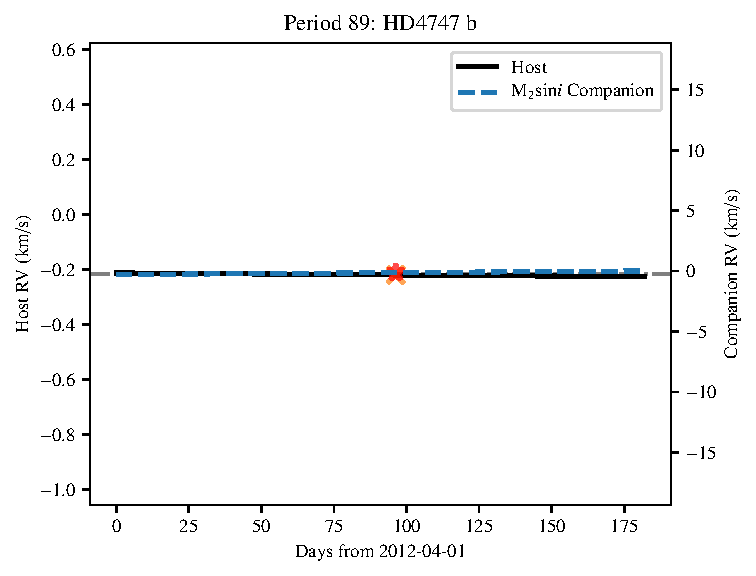
\includegraphics[width=0.45\linewidth]{figures/direct-recovery/orbital-plots/HD4747_p89.pdf}\\
    \end{tabular}
    \caption[]{{RV} single companion Keplerian orbit for {HD\,4747}.
        The left hand plot shows the {RV} curve for one full orbit while the right hand panel shows the {RV} curve over 6 months (Period 89).
        The solid black line indicates the {RV} of the host star (with scale on the left), while the blue dashed line indicates the {RV} of the companion (with scale on the right axis).
        The orange crosses and red stars indicate the times at which observations were obtained for the target, for the host and companion respectively.}
    \label{fig:hd4747p89}
\end{figure}

\begin{figure}
    \centering
    \begin{tabular}{cc}
        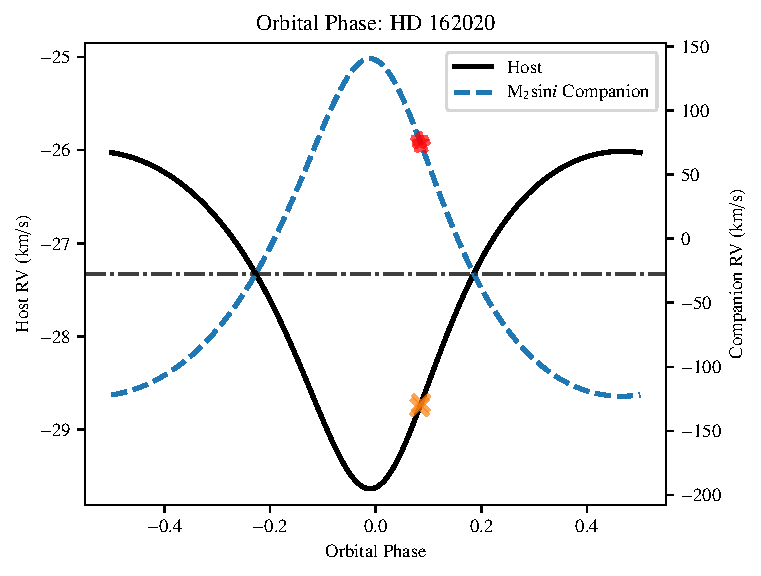
\includegraphics[width=0.45\linewidth]{figures/direct-recovery/orbital-plots/HD162020_orbital_phase.pdf} &
        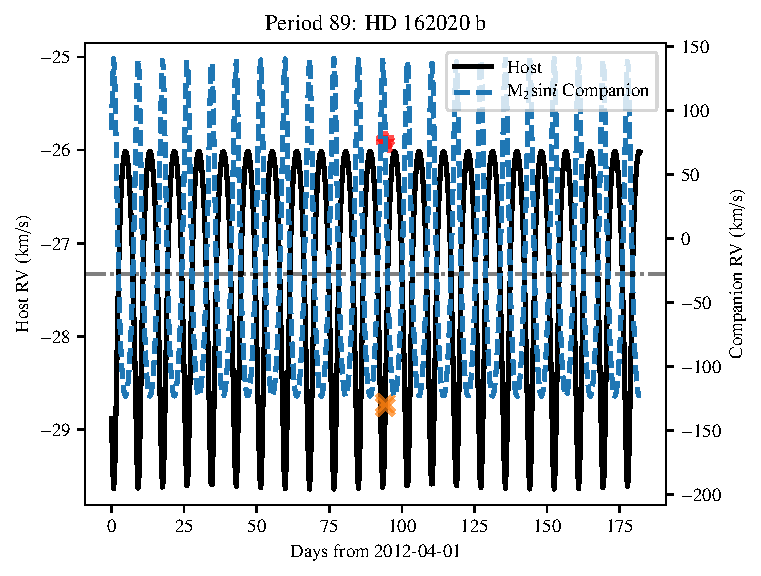
\includegraphics[width=0.45\linewidth]{figures/direct-recovery/orbital-plots/HD162020_p89.pdf}\\
    \end{tabular}
    \caption[]{Same as \cref{fig:hd4747p89} but for {HD\,162020}.}
    \label{fig:hd162020p89}
\end{figure}

\begin{figure}
    \centering
    \begin{tabular}{cc}
        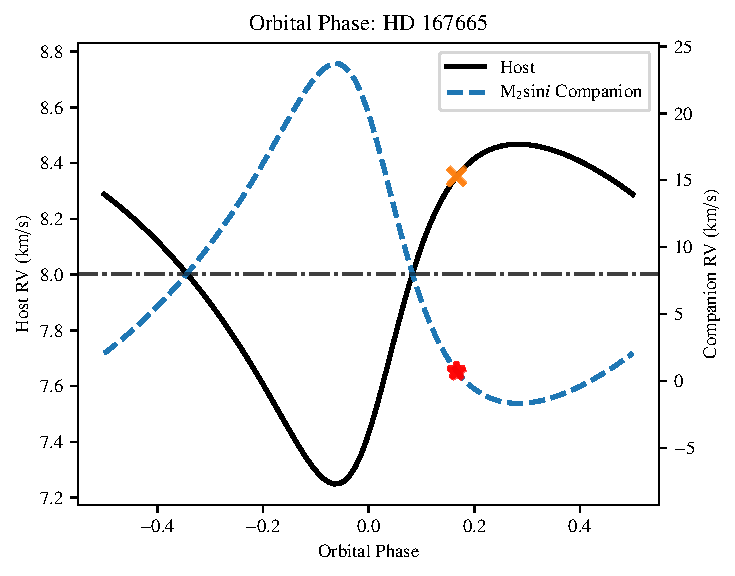
\includegraphics[width=0.45\linewidth]{figures/direct-recovery/orbital-plots/HD167665_orbital_phase.pdf} &
        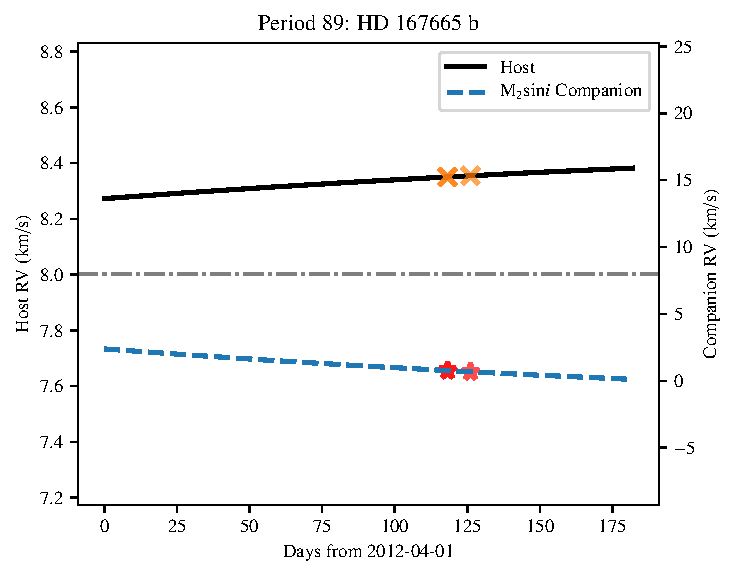
\includegraphics[width=0.45\linewidth]{figures/direct-recovery/orbital-plots/HD167665_p89.pdf}\\
    \end{tabular}
    \caption[]{Same as \cref{fig:hd4747p89} but for {HD\,167665}.}
    \label{fig:hd167665p89}
\end{figure}

\begin{figure}
    \centering
    \begin{tabular}{cc}
        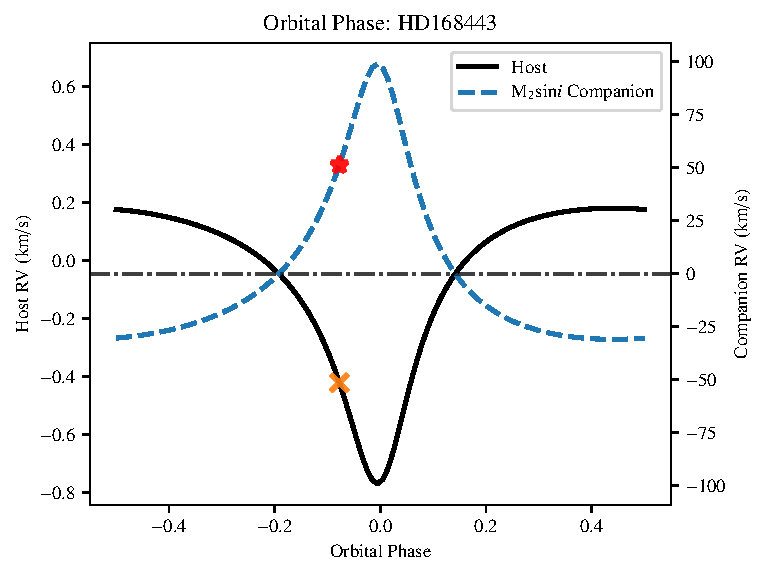
\includegraphics[width=0.45\linewidth]{figures/direct-recovery/orbital-plots/HD168443b_orbital_phase.pdf} &
        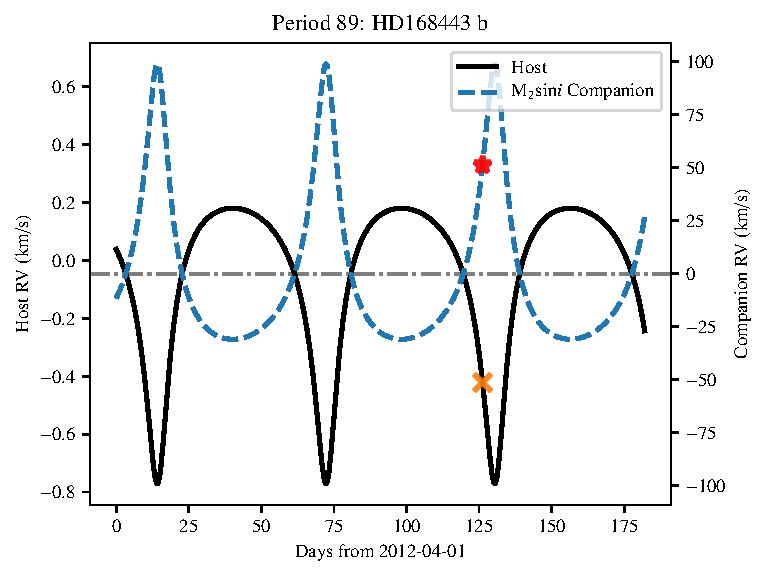
\includegraphics[width=0.45\linewidth]{figures/direct-recovery/orbital-plots/HD168443b_p89.pdf}\\
    \end{tabular}
    \caption[]{Same as \cref{fig:hd4747p89} but for {HD\,168443}b.
        Analysed as if this was a single companion.}
    \label{fig:hd168443bp89}
\end{figure}

\begin{figure}
    \centering
    \begin{tabular}{cc}
        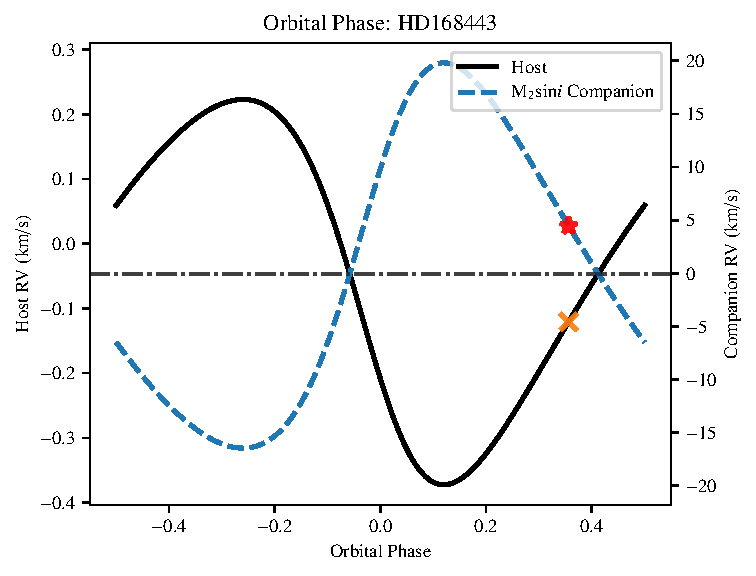
\includegraphics[width=0.45\linewidth]{figures/direct-recovery/orbital-plots/HD168443c_orbital_phase.pdf} &
        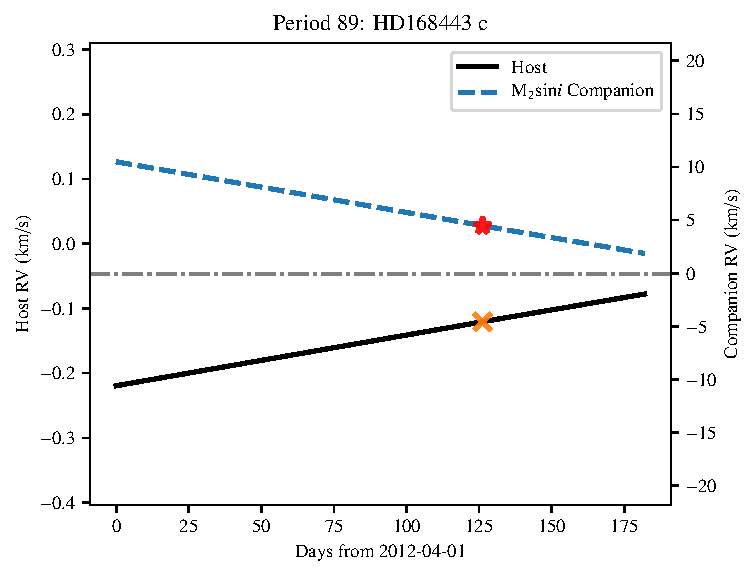
\includegraphics[width=0.45\linewidth]{figures/direct-recovery/orbital-plots/HD168443c_p89.pdf}\\
    \end{tabular}
    \caption[]{Same as \cref{fig:hd4747p89} but for {HD\,168443}c.
        Analysed as if this was a single companion.}
    \label{fig:hd168443cp89}
\end{figure}

\begin{figure}
    \centering
    \begin{tabular}{cc}
        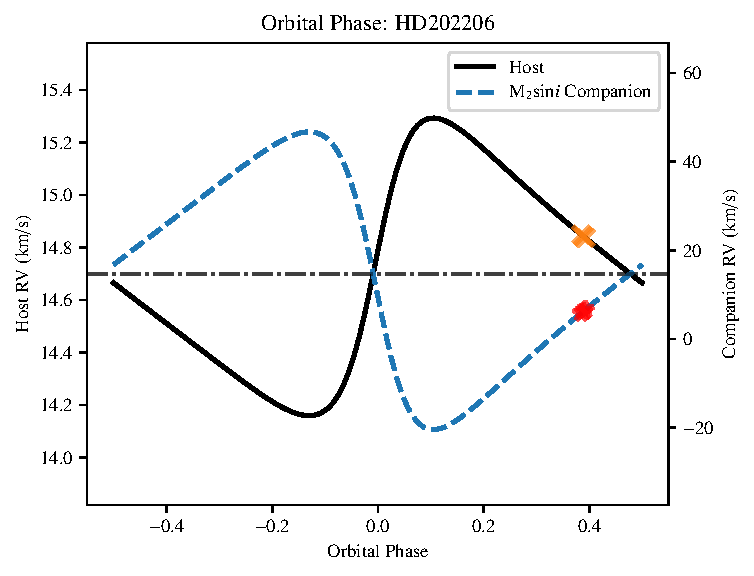
\includegraphics[width=0.45\linewidth]{figures/direct-recovery/orbital-plots/HD202206B_orbital_phase.pdf} &
        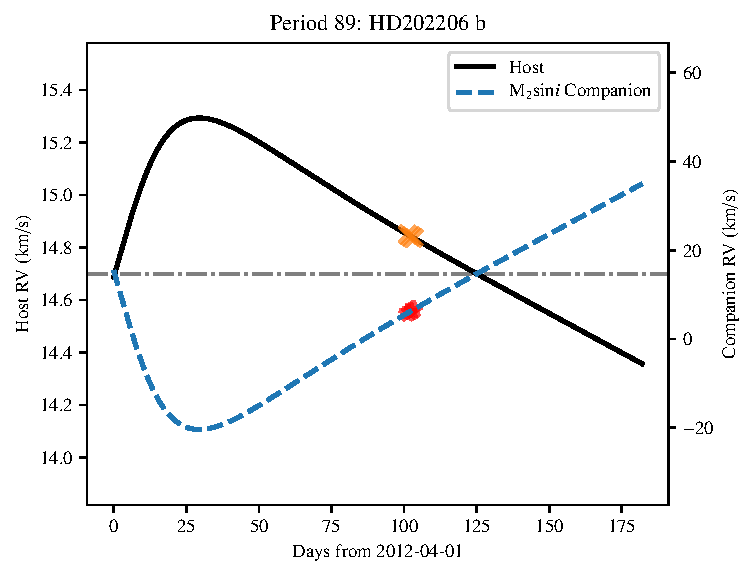
\includegraphics[width=0.45\linewidth]{figures/direct-recovery/orbital-plots/HD202206B_p89.pdf}\\
    \end{tabular}
    \caption[]{Same as \cref{fig:hd4747p89} but for {HD\,202206}B.
        Analysed as if this was a single companion.}
    \label{fig:hd202206bp89}
\end{figure}

\begin{figure}
    \centering
    \begin{tabular}{cc}
        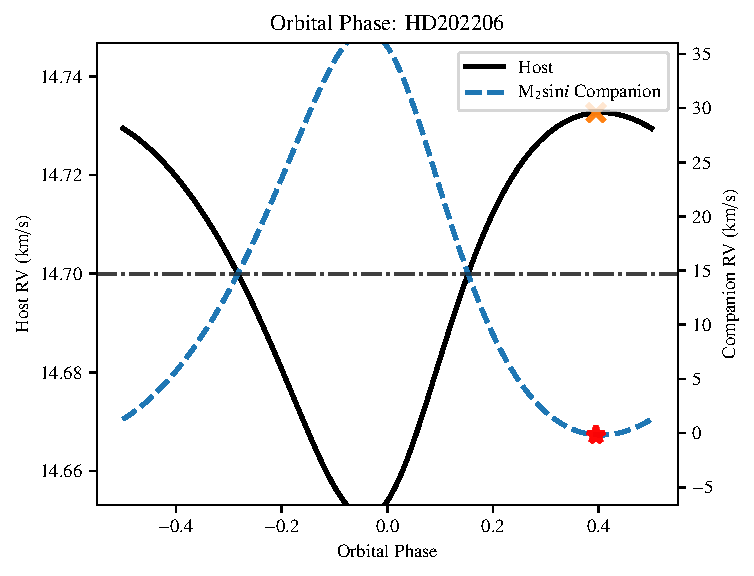
\includegraphics[width=0.45\linewidth]{figures/direct-recovery/orbital-plots/HD202206c_orbital_phase.pdf} &
        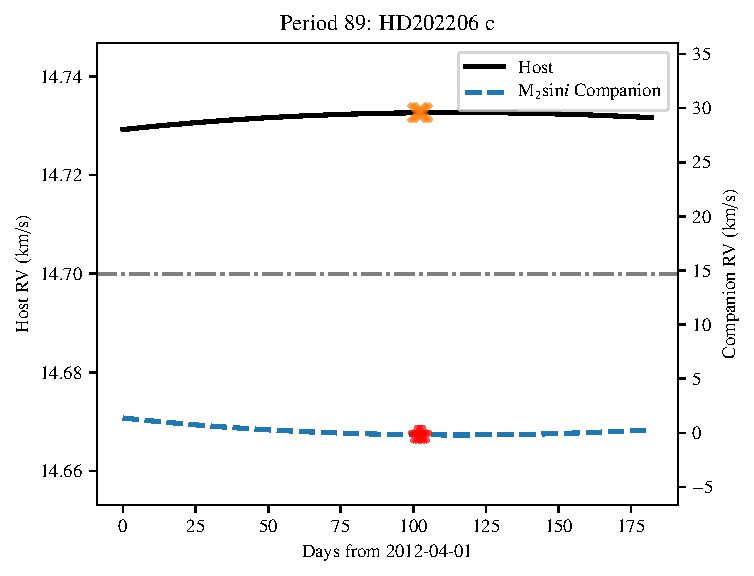
\includegraphics[width=0.45\linewidth]{figures/direct-recovery/orbital-plots/HD202206c_p89.pdf}\\
    \end{tabular}
    \caption[]{Same as \cref{fig:hd4747p89} but for {HD\,202206}c.
        Analysed as if this was a single companion.}
    \label{fig:hd202206cp89}
\end{figure}

\begin{figure}
    \centering
    \begin{tabular}{cc}
        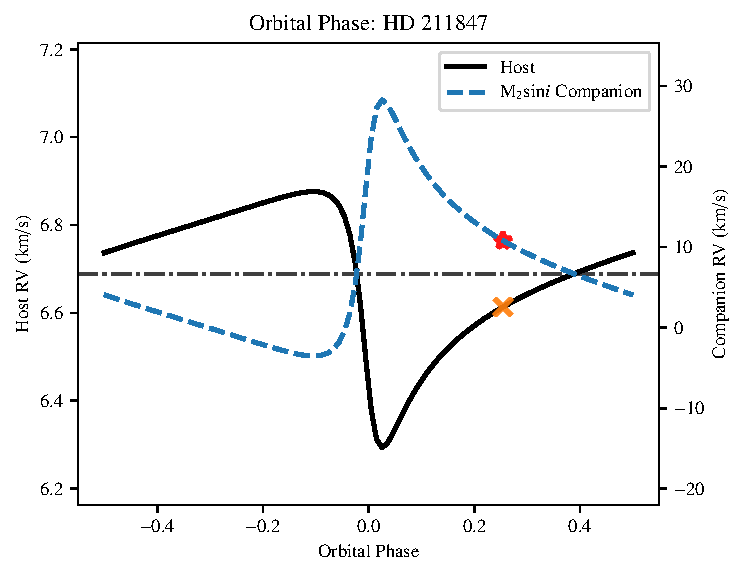
\includegraphics[width=0.45\linewidth]{figures/direct-recovery/orbital-plots/HD211847_orbital_phase.pdf} &
        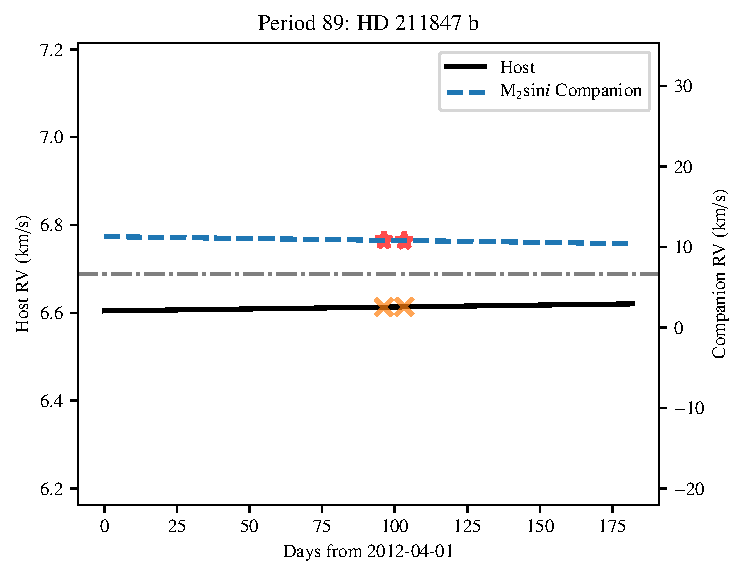
\includegraphics[width=0.45\linewidth]{figures/direct-recovery/orbital-plots/HD211847_p89.pdf}\\
    \end{tabular}
    \caption[]{Same as \cref{fig:hd4747p89} but for {HD\,211847}.}
    \label{fig:hd211847p89}
\end{figure}

\begin{figure}
    \centering
    \begin{tabular}{cc}
        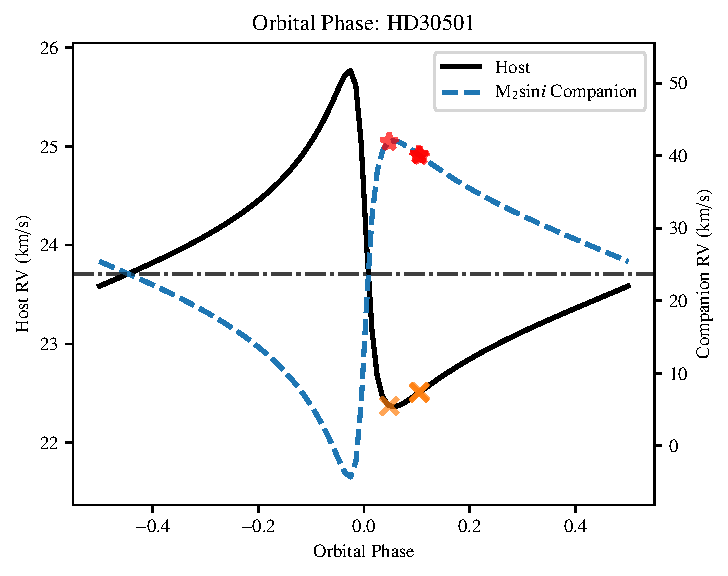
\includegraphics[width=0.45\linewidth]{figures/direct-recovery/orbital-plots/HD30501_orbital_phase.pdf} &
        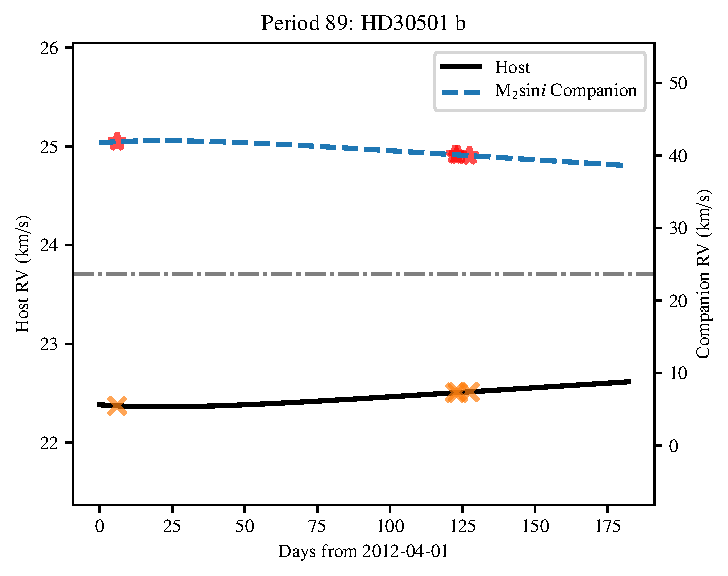
\includegraphics[width=0.45\linewidth]{figures/direct-recovery/orbital-plots/HD30501_p89.pdf}\\
    \end{tabular}
    \caption[]{Same as \cref{fig:hd4747p89} but for {HD\,30501}.}
    \label{fig:hd30501p89}
\end{figure}

% Add to list of figures.
\addtocontents{lof}{\protect\contentsline{figure}{\ref{fig:hd4747p89}--\ref{fig:hd30501p89} \quad {\color{hrefurlcolor} {RV} curves for the host and companion of each target.}}{{\color{black}\pageref{fig:hd4747p89}}}{}}


